\documentclass[11pt]{extarticle}
% Packages
\usepackage{algorithm}  
\usepackage{algorithmicx}  
\usepackage{algpseudocode}
\usepackage{amsmath}
\usepackage{amsthm}
\usepackage{amssymb}
\usepackage{amsfonts}
\usepackage{bm}
\usepackage{caption}
\usepackage{cite}
\usepackage{color}
\usepackage{enumerate}
\usepackage{framed}
\usepackage{graphicx}
\usepackage[hidelinks]{hyperref}
\hypersetup{
    colorlinks=true,
    linkcolor=blue,
    filecolor=magenta,
    urlcolor=cyan,
}
\urlstyle{same}
\usepackage{lipsum}
\usepackage{listings}
\usepackage{multirow}
\usepackage{subcaption}
% \usepackage{subfigure}
\usepackage{tikz}
\usepackage{titlesec}
\usepackage{xcolor}
\usepackage[english]{babel}
\usepackage[utf8]{inputenc}
\usepackage[normalem]{ulem}
\usepackage[top=1 in,bottom=1 in, left=1 in, right=1 in]{geometry}

\usepackage{pgfplots}
\pgfplotsset{compat=newest}
\usepgfplotslibrary{groupplots}
\usepgfplotslibrary{dateplot}

% Settings
\graphicspath{{./Figure/}}
\definecolor{mygreen}{rgb}{0,0.6,0}
\definecolor{mygray}{rgb}{0.5,0.5,0.5}
\definecolor{mymauve}{rgb}{0.58,0,0.82}
\definecolor{lightgray}{gray}{0.95}

\lstset{
    % backgroundcolor = \color{lightgray}, 
    basicstyle = \footnotesize,       
    breakatwhitespace = false,        
    breaklines = true,                 
    captionpos = b,                    
    commentstyle = \color{mygreen}\bfseries,
    emptylines = 1,
    escapeinside = @@,
    extendedchars = false,
    frame = single, 
    framerule = 0.5pt,
    keepspaces = true,
    keywordstyle = \color{mymauve}\bfseries,
    language = python,
    linewidth = \linewidth,
    numbers = left, 
    numbersep = 5pt,
    numberstyle = \tiny\color{mygray},
	otherkeywords = {string},    
    rulecolor = \color{black},         
    showspaces = false,  
    showstringspaces = false,
    showtabs = false,
    stepnumber = 5,         
    stringstyle = \color{mymauve},
    tabsize = 2,
    title = \lstname,
    %xleftmargin = 3em,
}

% A bunch of definitions that make my life easier
\newcommand{\A}{\mathbf{A}}
\newcommand{\D}{\mathcal{D}}
\newcommand{\E}{\mathbb{E}}
\newcommand{\I}{\mathbf{I}}
\newcommand{\N}{\mathcal{N}}
\renewcommand{\S}{\mathbf{S}}
\newcommand{\T}{\mathbf{T}}
\renewcommand{\t}{\mathbf{t}}
\newcommand{\W}{\mathbf{W}}
\newcommand{\w}{\mathbf{w}}
\newcommand{\X}{\mathbf{X}}
\newcommand{\x}{\mathbf{x}}
\newcommand{\Y}{\mathbf{Y}}
\newcommand{\y}{\mathbf{y}}
\newcommand{\Z}{\mathbf{Z}}
\newcommand{\0}{\mathbf{0}}

\renewcommand{\(}{\left(}
\renewcommand{\)}{\right)}

\DeclareMathOperator{\Beta}{Beta}
\DeclareMathOperator{\Bernoulli}{Bernoulli}
\DeclareMathOperator{\const}{const}
\DeclareMathOperator{\Dir}{Dir}
\DeclareMathOperator{\Gam}{Gam}
\DeclareMathOperator{\NormalGamma}{NormalGamma}
\DeclareMathOperator{\Poisson}{Poisson}
\DeclareMathOperator{\Tr}{Tr}

\renewcommand{\vec}{\mathrm{vec}}
\renewcommand{\emptyset}{\varnothing}
% \newcommand{\attn}[1]{\textbf{#1}}
\theoremstyle{definition}
\newtheorem{corollary}{Corollary}
\newtheorem{definition}{Definition}
\newtheorem{example}{Example}
\newtheorem{exercise}{Exercise}
\newtheorem{note}{Note}
\newtheorem{theorem}{Theorem}
\setlength{\columnseprule}{1 pt}
\renewcommand{\algorithmicrequire}{\textbf{Input:}}
\renewcommand{\algorithmicensure}{\textbf{Output:}}  
\newcommand{\image}[3]{
	\begin{figure}[!ht]
		\centering
	    \includegraphics[width=#1\textwidth]{#2}
		\caption{#3}
		\label{fig:#2}
	\end{figure}
}


\title{
    DD2434 Machine Learning, Advanced Course \\
    {\Large Assignment 1}
}
\author{
    Jiang, Sifan \\
	sifanj@kth.se \\
}


\begin{document}
\maketitle
\tableofcontents
\lstlistoflistings

\newpage
\section{Knowing the Rules}
\noindent\fcolorbox{black}{lightgray}{\begin{minipage}{\textwidth}
    \textbf{Question 2.1.1:} \textit{It is mandatory to read the above text. Have you read it?}
\end{minipage}} \\
\par Yes. \\

\noindent\fcolorbox{black}{lightgray}{\begin{minipage}{\textwidth}
    \textbf{Question 2.1.2:} \textit{List all your collaborations concerning the problem formulations in this assignment.}
\end{minipage}} \\
\par Hongsheng Chang. \\

\noindent\fcolorbox{black}{lightgray}{\begin{minipage}{\textwidth}
    \textbf{Question 2.1.3:} \textit{Have you discussed solutions with anybody?}
\end{minipage}} \\
\par No.


\section{Dependencies in a Directed Graphical Model}

%%%%% Question 2.2.4
\noindent\fcolorbox{black}{lightgray}{\begin{minipage}{\textwidth}
    \textbf{Question 2.2.4:} \textit{In the graphical model of Figure \ref{fig:Q2_2}, is $\mu_{k} \perp \tau_{k}$ (not conditioned by anything)?}
\end{minipage}} \\
\par Yes. \\
%\par Yes, $\mu_{k} \perp \tau_{k}$ is true.
%\begin{align*}
%    p(\mu_{k}, \tau_{k}) =& p(\mu_{k})p(\tau_{k})p\left(X^{1}, \cdots, X^{N} \mid \mu_{k}, \tau_{k}\right).
%\end{align*}
%\par Since none of the variables are observed, after ``marginalizing both sides of'' the above equation over $X^{1}, \cdots, X^{N}$ we obtain \cite{Bishop}:
%\begin{align*}
%    p(\mu_{k}, \tau_{k}) =& p(\mu_{k})p(\tau_{k}).
%\end{align*}
%\par So, $\mu_{k} \perp \tau_{k}$. \\

%%%%% Question 2.2.5
\noindent\fcolorbox{black}{lightgray}{\begin{minipage}{\textwidth}
    \textbf{Question 2.2.5:} \textit{In the graphical model of Figure \ref{fig:Q2_2}, is $\mu_{k} \perp \tau_{k} \mid X^{1}, \cdots, X^{N}$?}
\end{minipage}} \\
\par No. \\
%\par No, $\mu_{k} \perp \tau_{k} \mid X^{1}, \cdots, X^{N}$ is false.
%\begin{align*}
%    p(\mu_{k}, \tau_{k} \mid X^{1}, \cdots, X^{N}) =& \frac{p\left(\mu_{k}, \tau_{k}, X^{1}, \cdots, X^{N} \right)}{p\left(X^{1}, \cdots , X^{N} \right)} \\
%    =& \frac{p(\mu_{k})p(\tau_{k})p\left(X^{1},\cdots,X^{N} \mid \mu_{k}, \tau_{k}\right)}{p\left(X^{1}, \cdots, X^{N}\right)},
%\end{align*}
%which isn't factorized into the product $p(\mu_{k})p(\tau_{k})$, thus $\mu_{k} \perp \tau_{k} \mid X^{1}, \cdots, X^{N}$ is false. \\

%%%%% Question 2.2.6
\noindent\fcolorbox{black}{lightgray}{\begin{minipage}{\textwidth}
    \textbf{Question 2.2.6:} \textit{In the graphical model of Figure \ref{fig:Q2_2_6}, is $\mu \perp \beta^{'}$ (not conditioned by anything)?}
\end{minipage}} \\
\par Yes. \\

%%%%% Question 2.2.7
\noindent\fcolorbox{black}{lightgray}{\begin{minipage}{\textwidth}
    \textbf{Question 2.2.7:} \textit{In the graphical model of Figure \ref{fig:Q2_2_6}, is $\mu \perp \beta^{'} \mid X^{1}, \cdots, X^{N}$?}
\end{minipage}} \\
\par No. \\

%%%%% Question 2.2.8
\noindent\fcolorbox{black}{lightgray}{\begin{minipage}{\textwidth}
    \textbf{Question 2.2.8:} \textit{In the graphical model of Figure \ref{fig:Q2_2_6}, is $X^{n} \perp S^{n}$ (not conditioned by anything)?}
\end{minipage}} \\
\par No. \\

%%%%% Question 2.2.9
\noindent\fcolorbox{black}{lightgray}{\begin{minipage}{\textwidth}
    \textbf{Question 2.2.9:} \textit{In the graphical model of Figure \ref{fig:Q2_2_6}, is $X^{n} \perp S^{n} \mid \mu_{k}, \tau_{k}$?}
\end{minipage}} \\
\par No.


\section{Likelihood of a tree GM only for E level}


\newpage
\section{Simple VI}
%%%%% Question 2.4.12
\noindent\fcolorbox{black}{lightgray}{\begin{minipage}{\textwidth}
    \textbf{Question 2.4.12:} \textit{Implement the VI algorithm for the variational distribution in Equation (10.24) in Bishop.}
\end{minipage}} \\
\par From \textit{Bishop} \cite{Bishop}, the variational distribution is given by
\begin{align*}
    q(\mu, \tau) =& q_{\mu}(\mu) q_{\tau}(\tau) \\
    q_{\mu}(\mu) =& \N(\mu \mid \mu_{N}, \lambda_{N}^{-1}) \\
    q_{\tau}(\tau) =& \Gam(\tau \mid a_{N}, b_{N}),
\end{align*}
where
\begin{align*}
    \mu_{N} =& \frac{\lambda_{0}\mu_{0} + N\bar{x}}{\lambda_{0} + N} \\
    \lambda_{N} =& (\lambda_{0} + N) \mathbb{E}\left[\tau\right] \\
    a_{N} =& a_{0} + \frac{N}{2} \\
    b_{N} =& b_{0} + \frac{1}{2} \mathbb{E}_{\mu}\left[\sum_{n=1}^{N}(x_{n}-\mu)^{2} + \lambda_{0}(\mu-\mu_{0})^{2}\right] \\
    =& b_{0} - \left(\sum_{n=1}^{N}x_{n} + \lambda_{0}\mu_{0}\right)\mathbb{E}_{\mu}[\mu] + \frac{1}{2}\left(\sum_{n=1}^{N}x_{n}^{2} + \lambda_{0}\mu_{0}^{2} + (\lambda_{0} + N)\mathbb{E}_{\mu}[\mu^{2}]\right).
\end{align*}
\par Where
\begin{align*}
	\mathbb{E}_{\mu}[\mu] =& \mu_{N} \\
	\mathbb{E}_{\mu}[\mu^{2}] =& \frac{1}{\lambda_{N}} + \mu_{N}^{2} \\
	\mathbb{E}_{\tau}[\tau] =& \frac{a_{N}}{b_{N}}.
\end{align*}
\par Due to non-informative condition, we set $\mu_{0} = \lambda_{0} = a_{0} = b_{0} = 0$. Then the VI algorithm would be an iterative algorithm that start with a set of initial values of $\mu_N$, $\lambda_{N}$, $a_{N}$, and $b_{N}$. Then the values of $\mu_N$, $\lambda_{N}$, $a_{N}$, and $b_{N}$ should be updated to obtain a converging result of approximated posterior distribution. The algorithm is shown in the following code:
\lstinputlisting[caption=Simple VI.]{Code/2_4.py}

%%%%% Question 2.4.13
\noindent\fcolorbox{black}{lightgray}{\begin{minipage}{\textwidth}
    \textbf{Question 2.4.13:} \textit{What is the exact posterior?}
\end{minipage}} \\
\par Since gamma distribution is a conjugate prior of the normal distribution, the joint distribution of the Normal-Gamma distribution is
\begin{align*}
    p(\mu, \tau \mid \mu_{0}, \lambda_{0}, a_{0}, b_{0}) =& \frac{b_{0}^{a_{0}} \sqrt{\lambda_{0}}}{\Gamma(a_{0})\sqrt{2\pi}} \tau^{a_{0}-\frac{1}{2}} \exp\left[-b_{0}\tau\right] \exp\left[-\frac{ \lambda \tau(\mu - \mu_{0})^2}{2}\right] \\
    p(\mu, \tau) \propto& \tau^{a_{0}-\frac{1}{2}} \exp\left[-b_{0}\tau\right] \exp\left[-\frac{ \lambda \tau(\mu - \mu_{0})^2}{2}\right]
\end{align*}
\par According to Bayesian theorem, we have
\begin{align*}
	p(\mu, \tau \mid \D) \propto& p(\D \mid \mu, \tau) p(\mu, \tau),
\end{align*}
where $p(\D \mid \mu, \tau)$ is the likelihood of the data points which have such relationship:
\begin{align*}
	p(\D \mid \mu, \tau) =& \prod_{i=1}^{N} p(x_{i} \mid \mu, \tau) \\
	\propto& \prod_{i=1}^{N} \tau^{1/2} \exp\left[-\frac{\tau}{2}(x_{i} - \mu)^{2}\right] \\
	\propto& \tau^{N/2} \exp\left[-\frac{\tau}{2}\sum_{i=1}^{N}(x_{i} - \mu)^{2}\right] \\
	\propto& \tau^{N/2} \exp\left[-\frac{\tau}{2}\sum_{i=1}^{N}(x_{i} - \bar{x} + \bar{x} - \mu)^{2}\right] \\
	\propto& \tau^{N/2} \exp\left[-\frac{\tau}{2}\sum_{i=1}^{N}\((x_{i}-\bar{x})^{2}+(\bar{x}-\mu)^{2}\)\right] \\
	\propto& \tau^{N/2} \exp\left[-\frac{\tau}{2}\(Ns+N(\bar{x}-\mu)^{2}\)\right],
\end{align*}
where $\bar{x} = \frac{1}{N}\sum_{i=1}^{N}x_{i}$ and $s = \frac{1}{N}\sum_{i=1}^{N}(x_{i}-\mu)^{2}$. Thus the posterior can be written into \cite{Doing}
\begin{align*}
	p(\mu, \tau \mid \D) \propto& p(\D \mid \mu, \tau) p(\mu, \tau) \\
	\propto& \tau^{N/2} \exp\left[-\frac{\tau}{2}\(Ns+N(\bar{x}-\mu)^{2}\)\right] \tau^{a_{0}-\frac{1}{2}} \exp\left[-b_{0}\tau\right] \exp\left[-\frac{ \lambda \tau(\mu - \mu_{0})^2}{2}\right] \\
	\propto& \tau^{\frac{N}{2} + a_{0} - \frac{1}{2}} \exp\left[-\tau\left(\frac{1}{2}Ns + b_{0}\right)\right]\exp\left[-\frac{\tau}{2}\left(\lambda_{0}(\mu - \mu_{0})^{2} + N(\bar{x} - \mu)^{2}\right)\right].
\end{align*}
\par The exponent (except the $-\frac{\tau}{2}$) in the last exponential term can be simplified into
\begin{align*}
	\lambda_{0}(\mu - \mu_{0})^{2} + N(\bar{x} - \mu)^{2} =& \lambda_{0} \mu^{2} - 2\lambda_{0}\mu\mu_{0} + \lambda_{0}\mu_{0}^{2} + N\mu^{2} - 2N\bar{x}\mu + N\bar{x}^{2} \\
	=& (\lambda_{0} + N)\mu^{2} - 2(\lambda_{0}\mu_{0} + N\bar{x})\mu + \lambda_{0}\mu_{0}^{2} + N\bar{x}^{2} \\
	=& (\lambda_{0} + N)\left( \mu^{2} - 2\frac{\lambda_{0}\mu_{0} + N\bar{x}}{\lambda_{0} + N}\mu \right) + \lambda_{0}\mu_{0}^{2} + N\bar{x}^{2} \\
	=& (\lambda_{0} + N)\left( \mu - \frac{\lambda_{0}\mu_{0} + N \bar{x}}{\lambda_{0} + N} \right)^{2} + \lambda_{0}\mu_{0}^{2} + N\bar{x}^{2} - \frac{(\lambda_{0}\mu_{0} + N\bar{x})^{2}}{\lambda_{0} + N} \\
	=& (\lambda_{0} + N)\left( \mu - \frac{\lambda_{0}\mu_{0} + N\bar{x}}{\lambda_{0} + N} \right)^{2} + \frac{\lambda_{0}N(\bar{x} - \mu_{0})^{2}}{\lambda_{0} + N}.
\end{align*}
\par Insert the above equation into the posterior distribution, we have
\begin{align*}
	p(\mu, \tau \mid \D) \propto& \tau^{\frac{N}{2} + a_{0} - \frac{1}{2}} \exp\left[-\tau\left(\frac{1}{2}Ns + b_{0}\right)\right] \exp\left[-\frac{\tau}{2}\left( (\lambda_{0} + N)\left( \mu - \frac{\lambda_{0}\mu_{0} + N\bar{x}}{\lambda_{0} + N} \right)^{2} + \frac{\lambda_{0}N(\bar{x} - \mu_{0})^{2}}{\lambda_{0} + N} \right)\right] \\
	\propto& \tau^{\frac{N}{2} + a_{0} - \frac{1}{2}} \exp\left[-\tau\left(\frac{1}{2}Ns + b_{0} + \frac{\lambda_{0}N(\bar{x} - \mu_{0})^{2}}{2(\lambda_{0} + N)}\right)\right] \exp\left[-\frac{\tau}{2} (\lambda_{0} + N)\left( \mu - \frac{\lambda_{0}\mu_{0} + N\bar{x}}{\lambda_{0} + N} \right)^{2} \right],
\end{align*}
which is in the form of a Normal-Gamma distribution, thus the exact posterior is
\begin{align*}
	p(\mu, \tau \mid \D) =& \NormalGamma(\mu', \lambda', a', b') \\
	\mu' =& \frac{\lambda_{0}\mu_{0} + N\bar{x}}{\lambda_{0} + N} \\
	\lambda' =& \lambda_{0} + N \\
	a' =& a_{0} + \frac{N}{2} \\
	b' =& b_{0} + \frac{1}{2}\left(Ns + \frac{\lambda_{0}N(\bar{x} - \mu_{0})^{2}}{\lambda_{0} + N}\right).
\end{align*}

%%%%% Question 2.4.14
\noindent\fcolorbox{black}{lightgray}{\begin{minipage}{\textwidth}
    \textbf{Question 2.4.14:} \textit{Compare the inferred variational distribution with the exact posterior. Run the inference on data points drawn from iid Gaussians. Do this for three interesting cases and visualize the results. Describe the differences.}
\end{minipage}} \\
\begin{enumerate}
	\item In this case, the number of data set is $N = 10$ and the initial values are $b_{N} = 5$ and $\lambda_{N} = 5$. The result is shown in fig~\ref{fig:2_4_1}, where the true posterior distribution is shown by the colorful contour lines, while the approximated distribution given by the VI algorithm is shown in blue contour lines and red contour lines when reached convergence. The convergence criteria is that both of $b_{N}$ and $\lambda_{N}$ are converge to a given threshold.
	\begin{figure}[!ht]
		\centering
		\begin{subfigure}{.4\textwidth}
			\centering
			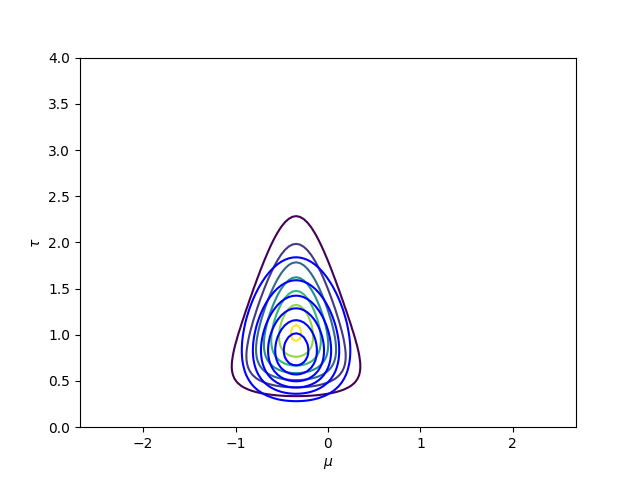
\includegraphics[width=\linewidth]{2_4_1_1}
		\end{subfigure}
		\begin{subfigure}{.4\textwidth}
			\centering
			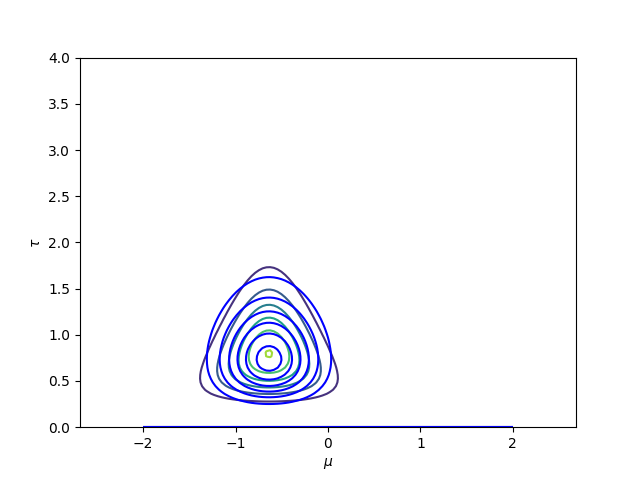
\includegraphics[width=\linewidth]{2_4_1_2}
		\end{subfigure}
		\begin{subfigure}{.4\textwidth}
			\centering
			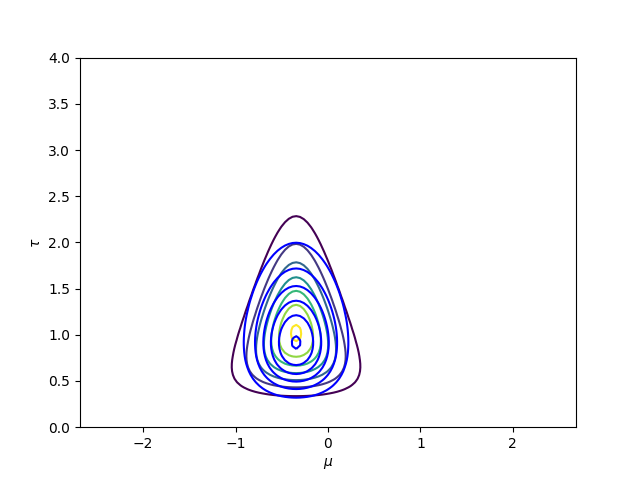
\includegraphics[width=\linewidth]{2_4_1_3}
		\end{subfigure}
		\begin{subfigure}{.4\textwidth}
			\centering
			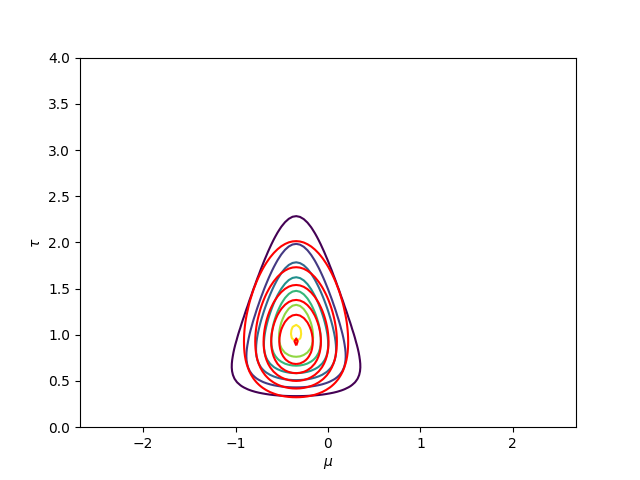
\includegraphics[width=\linewidth]{2_4_1_8}
		\end{subfigure}
		\caption{Simple VI with $\mu_{0} = \lambda_{0} = a_{0} = b_{0} = 0$, $b_{N} = 5$, and $\lambda_{N} = 5$ with $10$ samples.}
		\label{fig:2_4_1}
	\end{figure}
	\par Although we are using zero for parameters in the prior distributions, so that $\mu_{0} = \lambda_{0} = a_{0} = b_{0} = 0$, which implies that we have no information about the distribution, the convergence is really quick with VI algorithm, which is $8$ steps in my case.
	\par And not only from this case, but also from the following cases, we can see that the mean of the $\mu$ is always correct, which is true since we get value $\mu_{N}$ at the beginning and don't update it during the iterations.

	\item In this case, the number of data set is $N = 10$ and the initial values are $b_{N} = 0.1$ and $\lambda_{N} = 0.1$. The result is illustrated in fig~\ref{fig:2_4_2}.
	\begin{figure}[!ht]
		\centering
		\begin{subfigure}{.4\textwidth}
			\centering
			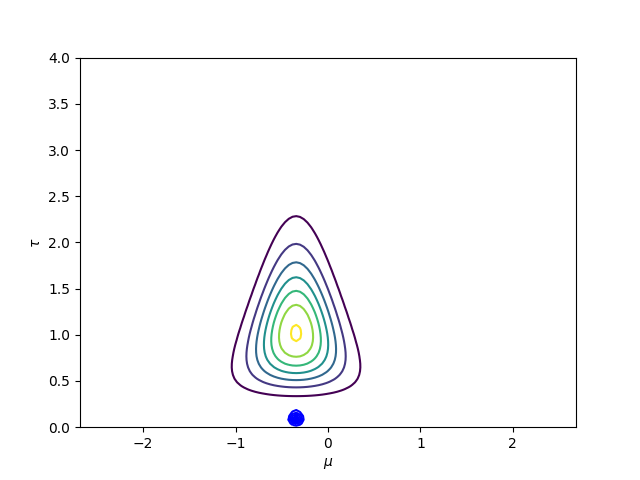
\includegraphics[width=\linewidth]{2_4_2_1}
		\end{subfigure}
		\begin{subfigure}{.4\textwidth}
			\centering
			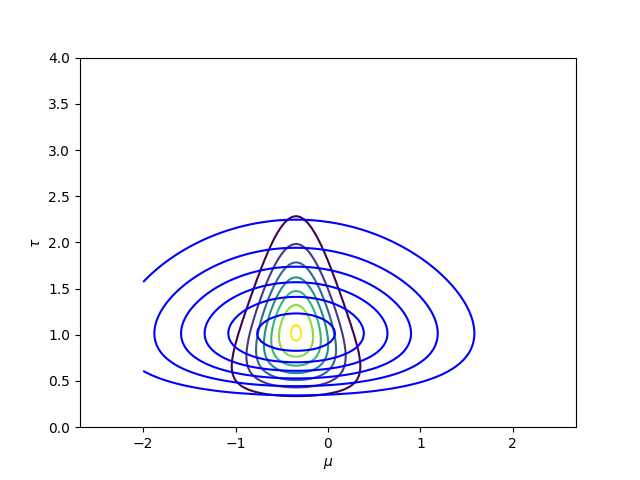
\includegraphics[width=\linewidth]{2_4_2_2}
		\end{subfigure}
		\begin{subfigure}{.4\textwidth}
			\centering
			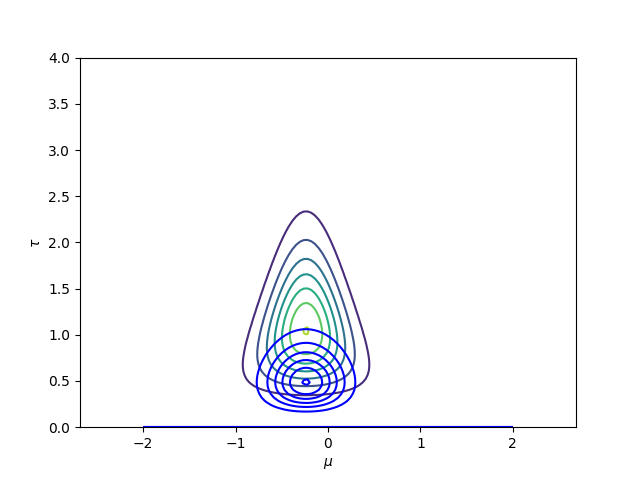
\includegraphics[width=\linewidth]{2_4_2_3}
		\end{subfigure}
		\begin{subfigure}{.4\textwidth}
			\centering
			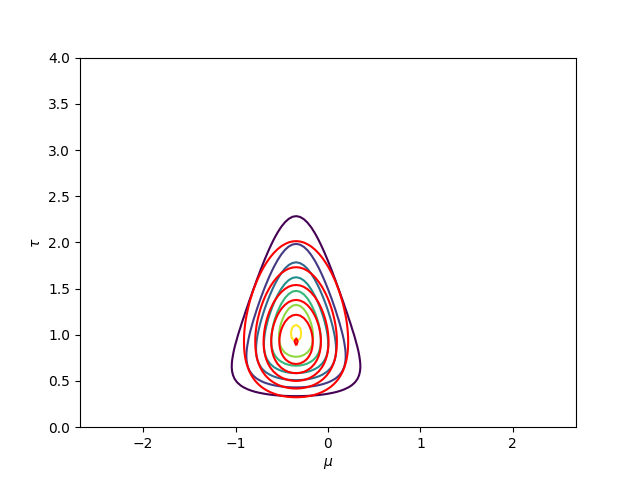
\includegraphics[width=\linewidth]{2_4_2_12}
		\end{subfigure}
		\caption{Simple VI with $\mu_{0} = \lambda_{0} = a_{0} = b_{0} = 0$, $b_{N} = 0.1$, and $\lambda_{N} = 0.1$ with $10$ samples.}
		\label{fig:2_4_2}
	\end{figure}
	\par By setting the value of the initial values $b_{N}$ and $\lambda_{N}$ to smaller values which are much different to the true values in the true posterior distribution, the converging procedure is slower and requires more iterations, in my case $12$ steps, to reach the convergence.
	
	\item In this case, the number of data set is $N = 100$ and the initial values are $b_{N} = 5$ and $\lambda_{N} = 5$. The result is illustrated in fig~\ref{fig:2_4_3}.
	\begin{figure}[!ht]
		\centering
		\begin{subfigure}{.4\textwidth}
			\centering
			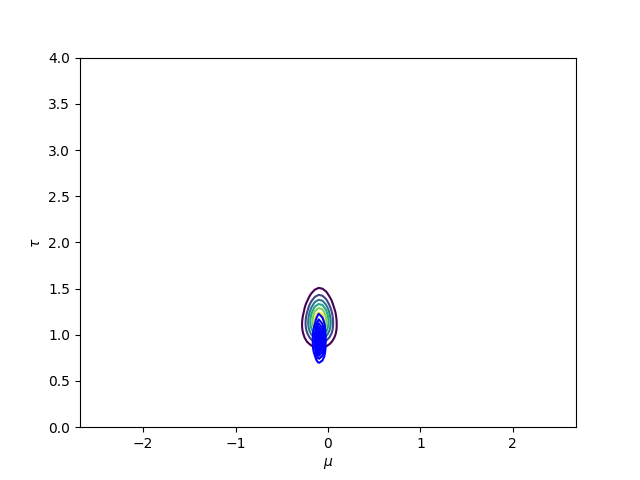
\includegraphics[width=\linewidth]{2_4_3_1}
		\end{subfigure}
		\begin{subfigure}{.4\textwidth}
			\centering
			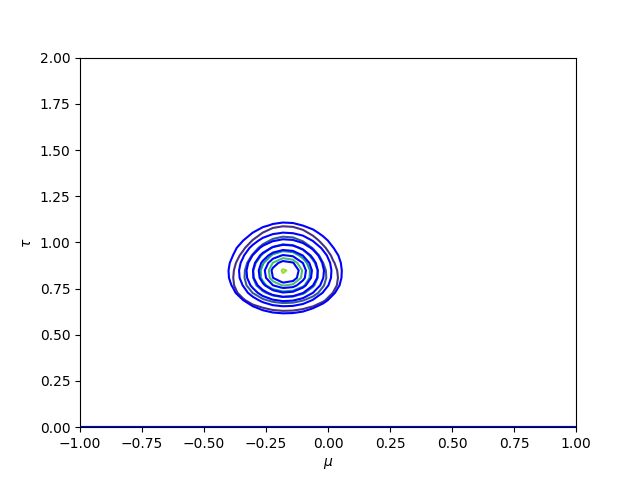
\includegraphics[width=\linewidth]{2_4_3_2}
		\end{subfigure}
		\begin{subfigure}{.4\textwidth}
			\centering
			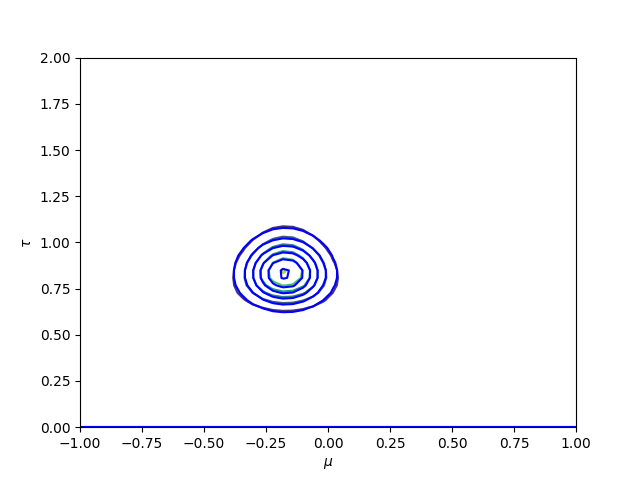
\includegraphics[width=\linewidth]{2_4_3_3}
		\end{subfigure}
		\begin{subfigure}{.4\textwidth}
			\centering
			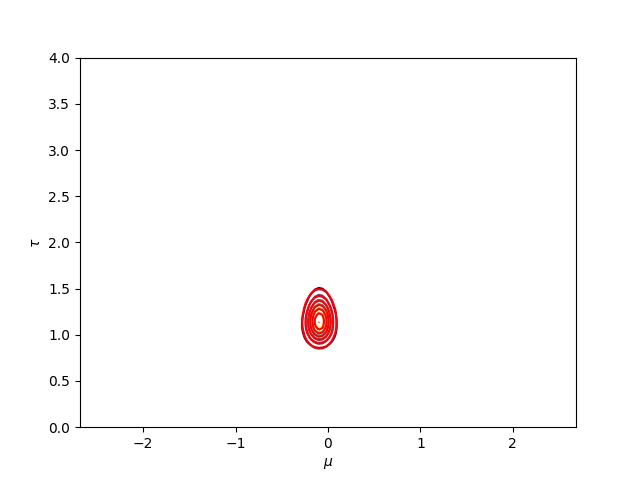
\includegraphics[width=\linewidth]{2_4_3_8}
		\end{subfigure}
		\caption{Simple VI with $\mu_{0} = \lambda_{0} = a_{0} = b_{0} = 0$, $b_{N} = 5$, and $\lambda_{N} = 5$ with $100$ samples.}
		\label{fig:2_4_3}
	\end{figure}
	\par In this case, we use $100$ data sets generated from a normal distribution. The true posterior distribution for $\mu$ and $\tau$ looks more like a circular shape. And since we have more data sets, we would be confident to the result and the convergence is quick at the same time, which is $8$ steps.
\end{enumerate}


\newpage
\section{Mixture of trees with observable variables}
%%%%% Question 2.5.15
\noindent\fcolorbox{black}{lightgray}{\begin{minipage}{\textwidth}
    \textbf{Question 2.5.15:} \textit{Implement this EM algorithm.}
\end{minipage}} \\
\par For each $n,k$ the responsibilities is
\begin{align*}
	r_{n,k} =& \frac{\pi_{k}p(x^{n} \mid T_{k}, \Theta_{k})}{p(x^{n})} \\
	=& \frac{\pi_{k}p(x^{n} \mid T_{k}, \Theta_{k})}{\sum_{k=1}^{K} \pi_{k}p(x^{n} \mid T_{k}, \Theta_{k})}.
\end{align*}
\par The algorithm is implemented below, where the function in \textit{Kruskal\_v1.py} is slightly modified so that the result of the maximum spanning tree can be returned:
\lstinputlisting[caption=EM algorithm for mixture of trees with observable variables.]{Code/2_5.py}

%%%%% Question 2.5.16
\noindent\fcolorbox{black}{lightgray}{\begin{minipage}{\textwidth}
    \textbf{Question 2.5.16:} \textit{Apply your algorithm to the provided data and show how well you reconstruct the mixtures. First, compare the real and inferred trees with the unweighted Robinson-Foulds (aka symmetric difference) metric. Do the trees have similar structure (don't worry if the inferred trees don't match with the real trees)? Then, compare the likelihoods of real and inferred mixtures. Finally, simulate more data and analyze the results (try to find some interesting and more challenging cases).}
\end{minipage}} \\
\begin{itemize}
	\item \textbf{\textit{q\_2\_5\_tm\_10node\_20sample\_4clusters}:} The result of the EM algorithm is illustrated in fig~\ref{fig:D10_N20_K4}.
	\image{0.9}{D10_N20_K4}{The likelihood and log-likelihood at each iteration of the EM algorithm for data \textit{q\_2\_5\_tm\_10node\_20sample\_4clusters}.}
	\par The comparison of the real and inferred trees with unweighted RF metric is show in tab~ \ref{tab:RF_D10_N20_K4}, from which we can see that the trees don't have similar structures which can caused by small number of samples.
	\begin{table}[!ht]
		\centering
		\caption{RF distance between the true tree mixture and the result obtained from the EM algorithm for data \textit{q\_2\_5\_tm\_10node\_20sample\_4clusters}, where the rows represents the obtained tree mixture and the columns represents the true tree mixture.}
		\begin{tabular}{c|cccc}
			 & 0 & 1 & 2 & 3 \\
			 \hline
			 0 & 9 & 8 & 10 & 10 \\
			 1 & 9 & 12 & 10 & 10 \\
			 2 & 8 & 7 & 9 & 9 \\
			 3 & 8 & 11 & 11 & 9
		\end{tabular}
		\label{tab:RF_D10_N20_K4}
	\end{table}
	\par The log-likelihood of the result tree mixture obtained by the EM algorithm is $-119.724756$, while the log-likelihood of the ground truth is $-113.143100$.
	\par Also, in the next question, $1000$ data points would be sampled from the tree mixture to see what would happen with the result of the EM algorithm.

	\item \textbf{\textit{q\_2\_5\_tm\_10node\_50sample\_4clusters}:} The result of the EM algorithm is illustrated in fig~\ref{fig:D10_N50_K4}.
	\image{0.9}{D10_N50_K4}{The likelihood and log-likelihood at each iteration of the EM algorithm for data \textit{q\_2\_5\_tm\_10node\_50sample\_4clusters}.}
	\par The comparison of the real and inferred trees with unweighted RF metric is show in tab~ \ref{tab:RF_D10_N50_K4}. Still the trees don't have similar structures but the distance looks more average than the one with only $20$ samples.
	\begin{table}[!ht]
		\centering
		\caption{RF distance between the true tree mixture and the result obtained from the EM algorithm for data \textit{q\_2\_5\_tm\_10node\_50sample\_4clusters}, where the rows represents the obtained tree mixture and the columns represents the true tree mixture.}
		\begin{tabular}{c|cccc}
			 & 0 & 1 & 2 & 3 \\
			 \hline
			 0 & 10 & 9 & 11 & 9 \\
			 1 & 11 & 8 & 10 & 10 \\
			 2 & 7 & 10 & 10 & 8 \\
			 3 & 10 & 9 & 9 & 11
		\end{tabular}
		\label{tab:RF_D10_N50_K4}
	\end{table}
	\par The log-likelihood of the result tree mixture obtained by the EM algorithm is $-416.226204$, while the log-likelihood of the ground truth is $-280.856624$.
	
	\item \textbf{\textit{q\_2\_5\_tm\_20node\_20sample\_4clusters}:} The result of the EM algorithm is illustrated in fig~\ref{fig:D20_N20_K4}.
	\image{0.9}{D20_N20_K4}{The likelihood and log-likelihood at each iteration of the EM algorithm for data \textit{q\_2\_5\_tm\_20node\_20sample\_4clusters}.}
	\par The comparison of the real and inferred trees with unweighted RF metric is show in tab~ \ref{tab:RF_D20_N20_K4}, from which we can see that the trees don't have similar structures which can caused by small number of samples and the result is even worse than the one with $10$ nodes due to the number of nodes is bigger, thus making the inference much harder and making it more difficult to have similar structures.
	\begin{table}[!ht]
		\centering
		\caption{RF distance between the true tree mixture and the result obtained from the EM algorithm for data \textit{q\_2\_5\_tm\_20node\_20sample\_4clusters}, where the rows represents the obtained tree mixture and the columns represents the true tree mixture.}
		\begin{tabular}{c|cccc}
			 & 0 & 1 & 2 & 3 \\
			 \hline
			 0 & 19 & 19 & 19 & 20 \\
			 1 & 19 & 19 & 19 & 22 \\
			 2 & 19 & 15 & 17 & 18 \\
			 3 & 18 & 20 & 24 & 21
		\end{tabular}
		\label{tab:RF_D20_N20_K4}
	\end{table}
	\par The log-likelihood of the result tree mixture obtained by the EM algorithm is $-278.687237$, while the log-likelihood of the ground truth is $-217.005755$.
\end{itemize}

%%%%% Question 2.5.17
\noindent\fcolorbox{black}{lightgray}{\begin{minipage}{\textwidth}
    \textbf{Question 2.5.17:} \textit{Simulate new tree mixtures with different number of nodes, samples and clusters. Try to find some interesting cases. Analyze your results as in the previous question.}
\end{minipage}} \\
\par By simulating a tree mixture with only $3$ nodes and $10$ clusters and sample $1000$ data points from the tree mixture, the result is shown in fig~\ref{fig:D3_N1000_K10}.
\image{0.9}{D3_N1000_K10}{The likelihood and log-likelihood at each iteration of the EM algorithm for tree mixture with $3$ nodes and $10$ clusters.}
\par The comparison of the real and inferred trees with unweighted RF metric is show in tab~ \ref{tab:RF_D3_N1000_K10}, from which we can see that the trees have similar structures because the number of nodes is only three which can be easily inferred.
	\begin{table}[!ht]
		\centering
		\caption{RF distance between the true tree mixture and the result obtained from the EM algorithm for tree mixture with $3$ nodes and $10$ clusters, where the rows represents the obtained tree mixture and the columns represents the true tree mixture.}
		\begin{tabular}{c|cccccccccc}
			  & 0 & 1 & 2 & 3 & 4 & 5 & 6 & 7 & 8 & 9 \\
			\hline
			0 & 2 & 2 & 0 & 0 & 2 & 0 & 2 & 2 & 0 & 2 \\
			1 & 2 & 2 & 0 & 0 & 2 & 0 & 2 & 2 & 0 & 2 \\
			2 & 2 & 2 & 0 & 0 & 2 & 0 & 2 & 2 & 0 & 2 \\
			3 & 0 & 0 & 2 & 2 & 0 & 2 & 0 & 0 & 2 & 0 \\
			4 & 2 & 2 & 0 & 0 & 2 & 0 & 2 & 2 & 0 & 2 \\
			5 & 0 & 0 & 2 & 2 & 0 & 2 & 0 & 0 & 2 & 0 \\
			6 & 2 & 2 & 0 & 0 & 2 & 0 & 2 & 2 & 0 & 2 \\
			7 & 0 & 0 & 2 & 2 & 0 & 2 & 0 & 0 & 2 & 0 \\
			8 & 0 & 0 & 2 & 2 & 0 & 2 & 0 & 0 & 2 & 0 \\
			9 & 2 & 2 & 0 & 0 & 2 & 0 & 2 & 2 & 0 & 2
		\end{tabular}
		\label{tab:RF_D3_N1000_K10}
	\end{table}
\par The log-likelihood of the result tree mixture obtained by the EM algorithm is $-1997.297679$, while the log-likelihood of the ground truth is $-2003.252791$.

\par Another example simulating a tree mixture with $10$ nodes and $10$ clusters, and sample $50$ data points from the tree mixture (notice that it is similar to \textit{q\_2\_5\_tm\_10node\_50sample\_4clusters} while the only difference is the number of clusters), the result of the EM algorithm is illustrated in fig~\ref{fig:D10_N50_K10}.
	\image{0.9}{D10_N50_K10}{The likelihood and log-likelihood at each iteration of the EM algorithm for tree mixture with $10$ nodes and $10$ clusters.}
	\par The comparison of the real and inferred trees with unweighted RF metric is show in tab~ \ref{tab:RF_D10_N50_K10}, from which we can see that the trees have more similar structures when compared to the case of \textit{q\_2\_5\_tm\_10node\_50sample\_4clusters}.
	\begin{table}[!ht]
		\centering
		\caption{RF distance between the true tree mixture and the result obtained from the EM algorithm for tree mixture with $10$ nodes and $10$ clusters, where the rows represents the obtained tree mixture and the columns represents the true tree mixture.}
		\begin{tabular}{c|cccccccccc}
			 & 0 & 1 & 2 & 3 & 4 & 5 & 6 & 7 & 8 & 9 \\
\hline
0 & 9 & 10 & 8 & 7 & 7 & 9 & 5 & 11 & 9 & 6 \\
1 & 10 & 9 & 7 & 12 & 10 & 6 & 8 & 10 & 8 & 9 \\
2 & 11 & 8 & 8 & 11 & 9 & 7 & 7 & 11 & 9 & 8 \\
3 & 10 & 9 & 7 & 10 & 8 & 10 & 6 & 12 & 8 & 7 \\
4 & 9 & 8 & 8 & 9 & 9 & 7 & 9 & 9 & 9 & 8 \\
5 & 10 & 9 & 9 & 10 & 12 & 10 & 10 & 10 & 10 & 11 \\
6 & 9 & 10 & 8 & 7 & 9 & 9 & 7 & 11 & 9 & 8 \\
7 & 10 & 7 & 7 & 8 & 8 & 8 & 8 & 10 & 8 & 7 \\
8 & 9 & 8 & 10 & 9 & 11 & 11 & 9 & 9 & 11 & 10\\
9 & 11 & 8 & 8 & 9 & 9 & 7 & 9 & 11 & 9 & 8
		\end{tabular}
		\label{tab:RF_D10_N50_K10}
	\end{table}
	\par The log-likelihood of the result tree mixture obtained by the EM algorithm is $-359.954244$, while the log-likelihood of the ground truth is $-323.847884$. Which are relatively similar when compare to the case of \textit{q\_2\_5\_tm\_10node\_50sample\_4clusters}.


\newpage
\section{Super epicentra - EM}
\image{0.5}{Q2_2}{Mixture of components modeling location and strengths of earthquakes associated with a super-epicentra. In the figure, $\mu_{k} = (\mu_{k,1}, \mu_{k,2})$ and $\tau_{k} = (\tau_{k,1}, \tau_{k,2})$.}
%%%%% Question 2.6.18
\noindent\fcolorbox{black}{lightgray}{\begin{minipage}{\textwidth}
    \textbf{Question 2.6.18:} \textit{Derive an EM algorithm for the model.}
\end{minipage}} \\
\par The conditional distribution of $X^{n}, S^{n}$ given a particular value for $Z^{n}$ is
\begin{align*}
	p(X^{n}, S^{n} \vert Z^{n}_{k}=1) =& \N(X^{n} \vert \mu_{k}, \tau_{k}) \mathrm{Poisson}(S^{n} \vert \lambda_{k}) \\ 
	=& \frac{\sqrt{\tau_{k,1}\tau_{k,2}}}{2\pi} \exp\left[-\frac{\tau_{k,1}}{2}(X^{n}_{1} - \mu_{k,1})^{2} - \frac{\tau_{k,2}}{2}(X^{n}_{2} - \mu_{k,2})^{2}\right] \frac{\lambda_{k}^{S^{n}}}{S^{n}!} \exp\left[-\lambda_{k}\right] \\
	=& \frac{\sqrt{\tau_{k,1}\tau_{k,2}}}{2\pi} \frac{\lambda_{k}^{S^{n}}}{S^{n}!} \exp\left[-\frac{\tau_{k,1}}{2}(X^{n}_{1} - \mu_{k,1})^{2} - \frac{\tau_{k,2}}{2}(X^{n}_{2} - \mu_{k,2})^{2} -\lambda_{k}\right]
\end{align*}
\par which can also be written in the form
\begin{align*}
	p(X^{n}, S^{n} \vert Z^{n}) = \prod_{k=1}^{K} p(X^{n}, S^{n} \vert Z^{n}_{k}=1)^{Z^{n}_{k}}.
\end{align*}
\par The joint distribution is given by
\begin{align*}
	p(X^{n}, S^{n}, Z^{n}) = p(Z^{n}) p(X^{n}, S^{n} \vert Z^{n}),
\end{align*}
and the marginal distribution of $X^{n}, S^{n}$ is then obtained by summing the joint distribution over all possible states of $Z^{n}$ to give
\begin{align*}
	p(X^{n}, S^{n}) = \sum_{k=1}^{K} \pi_{k} p(X^{n}, S^{n} \vert Z^{n}_{k}=1).
\end{align*}
\par Another quantity that will play an important role is the conditional probability of $Z^{n}$ given $X^{n}, S^{n}$. We shall use $\gamma(Z^{n}_{k})$ to denote $p(Z^{n}_{k} = 1 \vert X^{n}, S^{n})$, whose value can be found using Bayes' theorem
\begin{align*}
	\gamma(Z^{n}_{k}) \equiv p(Z^{n}_{k} = 1 \vert X^{n}, S^{n}) =& \frac{p(Z^{n}_{k}=1)p(X^{n}, S^{n} \vert Z^{n}_{k} = 1)}{\sum_{j=1}^{K}p(Z^{n}_{j}=1)p(X^{n}, S^{n} \vert Z^{n}_{j}=1)} \\
	=& \frac{\pi_{k} p(X^{n}, S^{n} \vert Z^{n}_{k} = 1)}{\sum_{j=1}^{K}\pi_{j} p(X^{n}, S^{n} \vert Z^{n}_{j}=1)}.
\end{align*}
\par The M-step in general EM algorithm is to evaluate $\bm{\theta}^{\mathrm{new}}$ given by
\begin{align*}
	\bm{\theta}^{\mathrm{new}} =& \arg_{\bm{\theta}}\max \mathcal{Q}(\bm{\theta}, \bm{\theta}^{\mathrm{old}})
\end{align*}
where
\begin{align*}
	\mathcal{Q}(\bm{\theta}, \bm{\theta}^{\mathrm{old}}) =& \sum_{\mathbf{Z}} p(\mathbf{Z} \vert \mathbf{X}, \mathbf{S}, \bm{\theta}^{\mathrm{old}}) \ln p(\mathbf{X}, \mathbf{S}, \mathbf{Z} \vert \bm{\theta}) \\
	=& \sum_{\mathbf{Z}} p(\mathbf{Z} \vert \mathbf{X}, \mathbf{S}, \bm{\theta}^{\mathrm{old}}) \ln p(\mathbf{Z} \vert \bm{\theta}) p(\mathbf{X}, \mathbf{S} \vert \mathbf{Z}, \bm{\theta})
\end{align*}
\par Setting the derivatives of $p(\Z \vert \X, \S, \bm{\theta}^{\mathrm{old}})\ln p(\X, \S, \Z \vert \bm{\theta})$ with respect to $\bm{\theta}$ to zero, we have the updated parameters given by
\begin{align*}
	\mu_{k}^{\mathrm{new}} =& \frac{1}{N_{k}} \sum_{n=1}^{N} \gamma(Z^{n}_{k}) X^{n} \\
	\tau_{k,1}^{\mathrm{new}} =& \frac{N_{k}}{\sum_{n=1}^{N} \gamma(Z^{n}_{k}) (X^{n}_{1} - \mu_{k,1}^{\mathrm{new}})^{2}} \\
	\tau_{k,2}^{\mathrm{new}} =& \frac{N_{k}}{\sum_{n=1}^{N} \gamma(Z^{n}_{k}) (X^{n}_{2} - \mu_{k,2}^{\mathrm{new}})^{2}} \\
	\lambda_{k}^{\mathrm{new}} =& \frac{1}{N_{k}} \sum_{n=1}^{N} \gamma(Z^{n}_{k}) S^{n} \\
	\pi_{k}^{\mathrm{new}} =& \frac{N_{k}}{N}.
\end{align*}

\par \textbf{EM algorithm:}
\begin{enumerate}
	\item Initialize the means $\mu_{k}$, precision $\tau_{k}$, Poisson parameter $\lambda_{k}$ and mixing coefficients $\pi_{k}$, and evaluate the initial value of the log likelihood.
	\item \textbf{E Step.} Evaluate the responsibilities using the current parameter values
	% \par Evaluate $p(\mathbf{Z} \vert \mathbf{X}, \mathbf{S}, \bm{\theta}^{\mathrm{old}})$
	\begin{align*}
		\gamma(Z^{n}_{k}) =& \frac{\pi_{k} p(X^{n}, S^{n} \vert Z^{n}_{k} = 1)}{\sum_{j=1}^{K}\pi_{j} p(X^{n}, S^{n} \vert Z^{n}_{j}=1)}.
	\end{align*}
	\item \textbf{M Step.} Re-estimate the parameters using the current responsibilities
	\begin{align*}
		\mu_{k}^{\mathrm{new}} =& \frac{1}{N_{k}} \sum_{n=1}^{N} \gamma(Z^{n}_{k}) X^{n} \\
		\tau_{k,1}^{\mathrm{new}} =& \frac{N_{k}}{\sum_{n=1}^{N} \gamma(Z^{n}_{k}) (X^{n}_{1} - \mu_{k,1}^{\mathrm{new}})^{2}} \\
		\tau_{k,2}^{\mathrm{new}} =& \frac{N_{k}}{\sum_{n=1}^{N} \gamma(Z^{n}_{k}) (X^{n}_{2} - \mu_{k,2}^{\mathrm{new}})^{2}} \\
		\lambda_{k}^{\mathrm{new}} =& \frac{1}{N_{k}} \sum_{n=1}^{N} \gamma(Z^{n}_{k}) S^{n} \\
		\pi_{k}^{\mathrm{new}} =& \frac{N_{k}}{N}
	\end{align*}
	where
	\begin{align*}
		N_{k} =& \sum_{n=1}^{N} \gamma(Z^{n}_{k}).
	\end{align*}
	\item Evaluate the log likelihood
	\begin{align*}
		\ln p(\X, \mathbf{S} \vert \bm{\mu}, \bm{\tau}, \bm{\lambda}, \bm{\pi}) = \sum_{n=1}^{N} \ln\left\{ \sum_{k=1}^{K} \pi_{k}\N(X^{n} \vert \mu_{k}, \tau_{k})\mathrm{Poisson}(S^{n} \vert \lambda_{k}) \right\}
	\end{align*}
	and check for convergence of either the parameters or the log likelihood. If the convergence criterion is not satisfied return to step 2.
\end{enumerate}


%%%%% Question 2.6.19
\noindent\fcolorbox{black}{lightgray}{\begin{minipage}{\textwidth}
    \textbf{Question 2.6.19:} \textit{Implement your EM algorithm.}
\end{minipage}} \\
\lstinputlisting[caption=EM algorithm for super epicentra.]{Code/2_6.py}

%%%%% Question 2.6.20
\noindent\fcolorbox{black}{lightgray}{\begin{minipage}{\textwidth}
    \textbf{Question 2.6.20:} \textit{Apply it to the data provided separately, give an account of the success, and provide visualizations for a couple of examples.}
\end{minipage}} \\
\begin{figure}[!ht]
	\centering
	\begin{subfigure}{.49\textwidth}
		\centering
		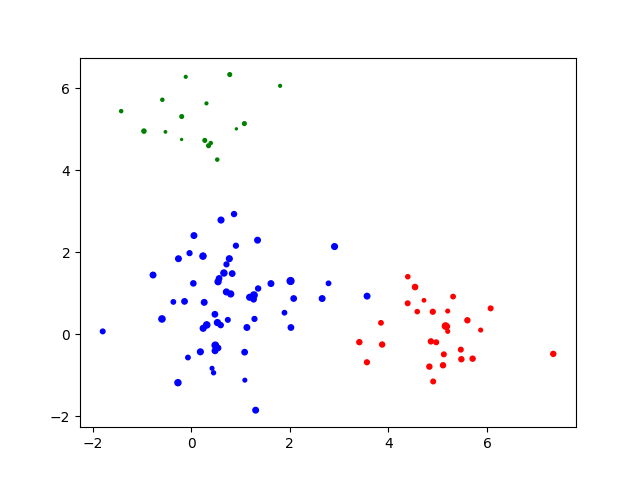
\includegraphics[width=\linewidth]{2_6_EM1}
		\caption{Data set 1.}
	\end{subfigure}
	\begin{subfigure}{.49\textwidth}
		\centering
		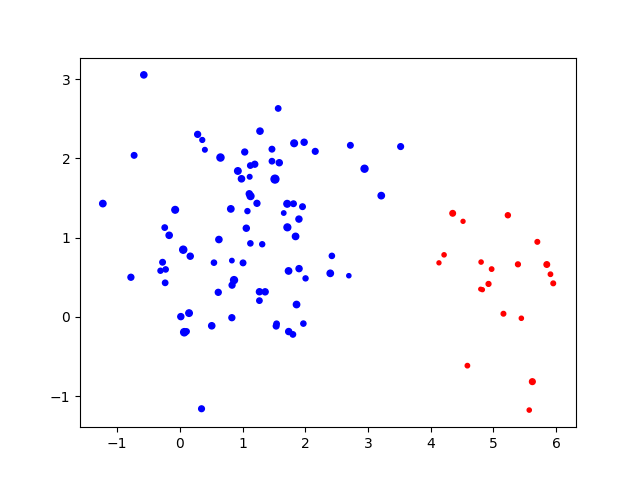
\includegraphics[width=\linewidth]{2_6_EM2}
		\caption{Data set 2.}
	\end{subfigure}
	\caption{Ground truth for data sets}
	\label{fig:2_6_Truth}
\end{figure}
\begin{figure}[!ht]
	\centering
	\begin{subfigure}{.49\textwidth}
		\centering
		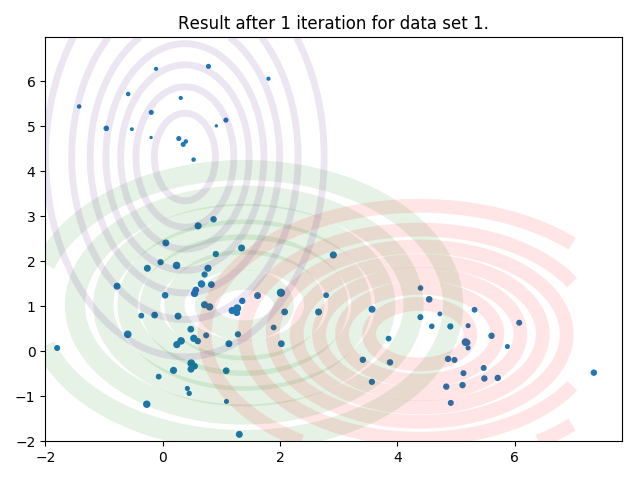
\includegraphics[width=\linewidth]{2_6_EM1_1}
	\end{subfigure}
	\begin{subfigure}{.49\textwidth}
		\centering
		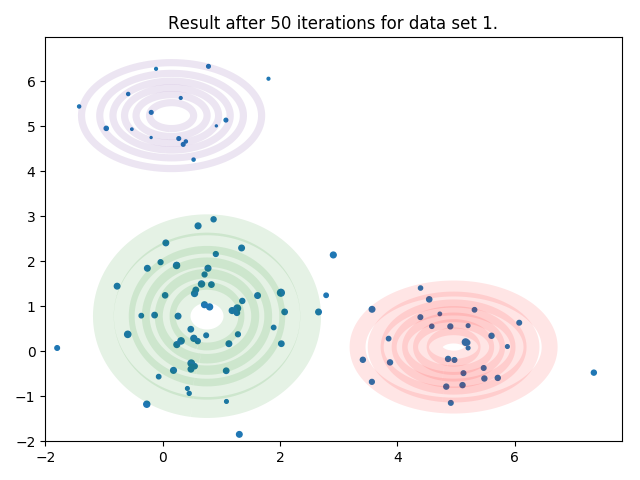
\includegraphics[width=\linewidth]{2_6_EM1_50}
	\end{subfigure}
	\begin{subfigure}{.49\textwidth}
		\centering
		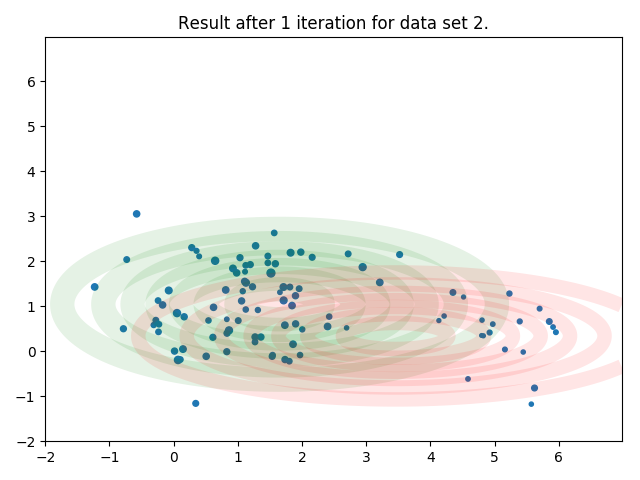
\includegraphics[width=\linewidth]{2_6_EM2_1}
	\end{subfigure}
	\begin{subfigure}{.49\textwidth}
		\centering
		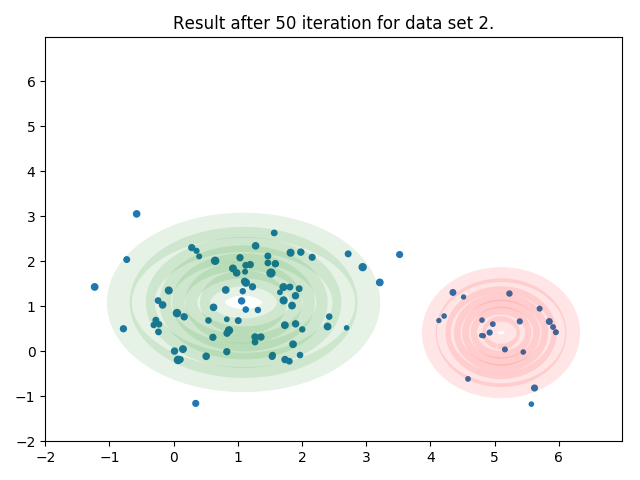
\includegraphics[width=\linewidth]{2_6_EM2_50}
	\end{subfigure}
	\caption{Result of the EM algorithm for different data sets.}
	\label{fig:2_6_Result}
\end{figure}
\par The ground truth of the data is illustrated in fig~\ref{fig:2_6_Truth} and the inference result from EM algorithm is illustrated in fig~\ref{fig:2_6_Result}. From those two figures, we can tell that the result of EM algorithm gives good inference of the means and covariances for each Gaussian model, and ratios for each Poisson model.


\section{Super epicentra - VI}
\image{0.5}{Q2_2_6}{The $K$ super epicentra model with priors.}
%%%%% Question 2.7.21
\noindent\fcolorbox{black}{lightgray}{\begin{minipage}{\textwidth}
    \textbf{Question 2.7.21:} \textit{Derive a VI algorithm that estimates the posterior distribution for this model.}
\end{minipage}} \\
\par The VI algorithm is derived based on \cite{Bishop} and lecture notes.
\par Since $\pi \sim \mathrm{Dir}(\alpha)$, we have
\begin{align*}
	p(\pi \vert \alpha) =& p(\pi_{1}, \cdots, \pi_{K} \vert \alpha_{1}, \cdots, \alpha_{K}) \\
	=& \frac{\Gamma\left(\sum_{k=1}^{K} \alpha_{k}\right)}{\prod_{k=1}^{K}\Gamma(\alpha_{k})} \prod_{k=1}^{K} \pi_{k}^{\alpha_{k}-1} \\
	=& \frac{1}{B(\alpha)} \prod_{k=1}^{K} \pi_{k}^{\alpha_{k}-1}.
\end{align*}
\par Also, for other latent variables, we have
\begin{align*}
	p(\mu_{k} \vert \tau_{k}) =& \N(\mu_{k} \vert \mu, (C \tau_{k})^{-1}) \\
	p(\tau_{k}) =& \Gam(\tau_{k} \vert \alpha', \beta') \\
	p(\lambda_{k}) =& \Gam(\lambda_{k} \vert \alpha_{0}, \beta_{0}).
\end{align*}
\par The joint distribution of all of the random variables is given by
\begin{align*}
	p(\X, \S, \Z, \pi, \mu, \tau, \lambda) = p(\X|\Z,\mu,\tau) p(\S|\Z,\lambda) p(\Z|\pi) p(\pi) p(\mu|\tau) p(\tau) p(\lambda).
\end{align*}
\par A variational distribution which factorizes between the latent variables and the parameters is given by
\begin{align*}
	q(\Z, \pi, \mu, \tau, \lambda) = q(\Z) q(\pi, \mu, \tau, \lambda).
\end{align*}
\par The log of the optimized factor is then given by
\begin{align*}
	\ln q^{*}(\Z) =& \mathbb{E}_{\pi, \mu, \tau, \lambda}[\ln p(\X, \S, \Z, \pi, \mu, \tau, \lambda)] + \const \\
	=& \mathbb{E}_{\pi}[\ln p(\Z \vert \pi)] + \mathbb{E}_{\mu, \tau}[\ln p(\X \vert \Z, \mu, \tau)] + \mathbb{E}_{\lambda}[\ln p(\S \vert \Z, \lambda)] + \const \\
	=& \sum_{n=1}^{N}\sum_{k=1}^{K} Z^{n}_{k} \ln \rho_{nk} + \const
\end{align*}
where
\begin{align*}
	\ln \rho_{nk} =& \mathbb{E}\left[\ln \pi_{k}\right] + \frac{1}{2}\E\left[\ln\vert\tau_{k}\vert\right] - \ln(2\pi) \\ & - \frac{1}{2} \E_{\mu_{k}, \tau_{k}}\left[ (X^{n} - \mu_{k})^{\mathrm{T}}\tau_{k}(X^{n} - \mu_{k}) \right] \\ & + S^{n} \mathbb{E}[\ln \lambda_{k}] - \mathbb{E}[\lambda_{k}] - \ln\left(S^{n}!\right).
\end{align*}
\par Taking the exponential of both sides of the equation and normalize it, we obtain
\begin{align*}
	q^{*}(\Z) = \prod_{n=1}^{N}\prod_{k=1}^{K} r_{nk}^{Z^{n}_{k}}
\end{align*}
where
\begin{align*}
	r_{nk} = \frac{\rho_{nk}}{\sum_{j=1}^{K}\rho_{nj}}.
\end{align*}
\par For the discrete distribution $q^{*}(\Z)$ we have
\begin{align*}
	\mathbb{E}[Z^{n}_{k}] = r_{nk}
\end{align*}
and define 
\begin{align*}
	N_{k} =& \sum_{n=1}^{N} r_{nk}.
\end{align*}
\par Then consider the factor $q(\pi, \mu, \tau, \lambda)$ in the variational posterior distribution, we have
\begin{align*}
	\ln q^{*}(\pi, \mu, \tau, \lambda) =& \ln p(\pi) + \mathbb{E}_{\Z}[\ln p(\Z \vert \pi)] + \const \\ & + \sum_{k=1}^{K}\ln p(\mu_{k}, \tau_{k}) + \sum_{k=1}^{K}\sum_{n=1}^{N} \mathbb{E}[Z^{n}_{k}]\ln \N(X^{n} \vert \mu_{k}, \tau_{k}^{-1}) \\ & + \sum_{k=1}^{K}\ln p(\lambda_{k}) + \sum_{k=1}^{K}\sum_{n=1}^{N}\mathbb{E}[Z^{n}_{k}]\ln\Poisson(S^{n} \vert \lambda_{k}).
\end{align*}
\par Since the right-hand side of this expression decomposes into a sum of terms involving only $\pi$, terms only involving $\mu$ and $\tau$, and terms only involving $\lambda$, which implies that the variational posterior $q(\pi, \mu, \tau, \lambda)$ factorizes to give $q(\pi)q(\mu, \tau)q(\lambda)$ which gives
\begin{align*}
	q(\pi, \mu, \tau, \lambda) = q(\pi) \prod_{k=1}^{K} q(\mu_{k}, \tau_{k}) q(\lambda_{k}).
\end{align*}
\begin{itemize}
\item First, by identifying the terms that depend on $\pi$, we have
\begin{align*}
	\ln q^{*}(\pi) = (\alpha - 1) \sum_{k=1}^{K}\ln \pi_{k} + \sum_{k=1}^{K}\sum_{n}^{N}r_{nk}\ln \pi_{k} + \const
\end{align*}
and taking the exponential of both sides, we have
\begin{align*}
	q^{*}(\pi) = \Dir(\pi \vert \alpha^{*})
\end{align*}
where $\alpha^{*}$ has components $\alpha^{*}_{k}$ given by
\begin{align*}
	\alpha^{*}_{k} = \alpha_{k} + N_{k}.
\end{align*}

\item Similarly, by identifying the terms that depends on $\mu_{k}$ and $\tau_{k}$, we have
\begin{align*}
	\ln q^{*}(\mu_{k}, \tau_{k}) =& \sum_{n=1}^{N}r_{nk}\left(\frac{1}{2}\ln\tau_{k}-\frac{1}{2}\tau_{k}\left(X^{n}-\mu_{k}\right)^{2}\right) \\ & + \frac{1}{2}\ln\tau_{k} - \frac{1}{2}C(\mu_{k} - \mu)^{2} \\ & + (\alpha'-1)\ln\tau_{k} - \beta'\tau_{k}.
\end{align*}
So, we have
\begin{align*}
	q^{*}(\mu_{k} \vert \tau_{k}) =& \N(\mu_{k} \vert \mu^{*}, \tau^{*}) \\
	\tau^{*} =& (C + N_{k})\tau_{k} \\
	\mu^{*} =& \frac{\left(\tau_{k} \sum_{n=1}^{N} r_{nk}X^{n}\right) + C\tau_{k}\mu}{\tau^{*}},
\end{align*}
and
\begin{align*}
	q^{*}(\tau_{k}) =& \Gam(\tau_{k} \vert \alpha'^{*}, \beta'^{*}) \\
	\alpha'^{*} =& \alpha' + N_{k} \\
	\beta'^{*} =& \beta' + \frac{1}{2}C\mu^{2} + \frac{1}{2}\sum_{n=1}^{N}r_{nk}{X^{n}}^{2}.
\end{align*}

\item Finally, by identifying the terms that depends on $\lambda_{k}$, we have
\begin{align*}
	\ln q^{*}(\lambda_{k}) =& (\alpha_{0}-1)\ln\lambda_{k} - \beta_{0}\lambda_{k} + \const \\ & + \sum_{n=1}^{N}\left(r_{nk}\left(S^{n}\ln\lambda_{k} - \lambda_{k} - \ln \left(S^{n}!\right)\right)\right).
\end{align*}
So, we have
\begin{align*}
	q^{*}(\lambda_{k}) =& \Gam(\lambda_{k} \vert \alpha_{0}^{*}, \beta_{0}^{*}) \\
	\alpha_{0}^{*} =& \alpha_{0} + \sum_{n=1}^{N} r_{nk}S^{n} \\
	\beta_{0}^{*} =& \beta + N_{k}.
\end{align*}
\end{itemize}


\newpage
\section{Sampling from a tree GM}
%%%%% Question 2.8.22
\noindent\fcolorbox{black}{lightgray}{\begin{minipage}{\textwidth}
    \textbf{Question 2.8.22:} \textit{Derive these algorithms.}
\end{minipage}} \\
\begin{enumerate}
\item \textbf{Bottom-up Dynamic Programming (DP) algorithm:}
\par Define $\mathfrak{O}\{T\}$ such that the sum of the leaves of tree $T$ is odd. Similarly, define $\mathfrak{E}\{T\}$ such that the sum of the leaves of tree $T$ is even. Also, define $\mathcal{L}(T)$ to be the left subtree of the root of the tree $T$, and define $\mathcal{R}(T)$ to be the right subtree of the root of the tree $T$, which both can be empty tree. Then for an arbitrary tree, we have
\begin{align*}
	p(\mathfrak{O}\{T\} \vert T, \Theta) =& p(\mathfrak{O}\{\mathcal{L}(T)\} \vert \mathcal{L}(T), \Theta) p(\mathfrak{E}\{\mathcal{R}(T)\} \vert \mathcal{R}(T), \Theta) \\
	+&  p(\mathfrak{E}\{\mathcal{L}(T)\} \vert \mathcal{L}(T), \Theta) p(\mathfrak{O}\{\mathcal{R}(T)\} \vert \mathcal{R}(T), \Theta) \\
	p(\mathfrak{E}\{T\} \vert T, \Theta) =& p(\mathfrak{O}\{\mathcal{L}(T)\} \vert \mathcal{L}(T), \Theta) p(\mathfrak{O}\{\mathcal{R}(T)\} \vert \mathcal{R}(T), \Theta) \\
	+&  p(\mathfrak{E}\{\mathcal{L}(T)\} \vert \mathcal{L}(T), \Theta) p(\mathfrak{E}\{\mathcal{R}(T)\} \vert \mathcal{R}(T), \Theta) \\
\end{align*}
\par So, the recursions pertinent for getting an odd-sum output is to calculate both of: 
\begin{enumerate}[i]
\item the odd-sum output of left subtree and the even-sum output of right subtree;
\item the even-sum output of left subtree and the odd-sum output of right subtree.
\end{enumerate}
\par And the recursions pertinent for getting an even-sum output is to calculate both of:
\begin{enumerate}[i]
\item the odd-sum output of left subtree and the odd-sum output of right subtree;
\item the even-sum output of left subtree and the even-sum output of right subtree.
\end{enumerate}
\par And for a single step, the marginal probability is calculated, such that
\begin{align*}
	p(\mathfrak{O}\{T\} \vert T, \Theta) = \sum_{k=1}^{K} p(\mathfrak{O}\{T\}, X_{r(T)}=k \vert T, \Theta)
\end{align*}
where $X_{r(T)}$ means the root of the tree $T$.

\item \textbf{Top-down sampling algorithm:} To sample the leaves that with odd sum, we begin with sample the root with Bayesian theorem so that (for simplicity, $T$ and $\Theta$ are omitted)
\begin{align*}
	p(X_{r(T)} \vert \mathfrak{O}\{T\}) = \frac{p(\mathfrak{O}\{T\} \vert X_{r(T)}) p(X_{r(T)})}{p(\mathfrak{O}\{T\})}.
\end{align*}
\par Then, for the children of the root node, we would have two situations
\begin{align*}
	 & p(X_{r(\mathcal{L}(T))} \vert \mathfrak{O}\{\mathcal{L}(T)\}, X_{r(T)}) \; p(X_{r(\mathcal{R}(T))} \vert \mathfrak{E}\{\mathcal{R}(T)\}, X_{r(T)})
\end{align*}
and
\begin{align*}
	 & p(X_{r(\mathcal{L}(T))} \vert \mathfrak{O}\{\mathcal{L}(T)\}, X_{r(T)}) \; p(X_{r(\mathcal{R}(T))} \vert \mathfrak{O}\{\mathcal{R}(T)\}, X_{r(T)}).
\end{align*}
\par Then take one term as the example, we have
\begin{align*}
	p(X_{r(\mathcal{L}(T))} \vert \mathfrak{O}\{\mathcal{L}(T)\}, X_{r(T)}) & = \frac{p(\mathfrak{O}\{\mathcal{L}(T)\} \vert X_{r(\mathcal{L}(T))}) \; p(X_{r(\mathcal{L}(T))} \vert X_{r(T)})}{p(\mathfrak{O}\{\mathcal{L}(T)\} \vert X_{r(T)})}
\end{align*}
\end{enumerate}

%%%%% Question 2.8.23
\noindent\fcolorbox{black}{lightgray}{\begin{minipage}{\textwidth}
    \textbf{Question 2.8.23:} \textit{Implement your bottom up DP algorithm for the probability of generating an odd sum output.}
\end{minipage}} \\
\lstinputlisting[caption=Tree DP.]{Code/2_8_DP.py}

%%%%% Question 2.8.24
\noindent\fcolorbox{black}{lightgray}{\begin{minipage}{\textwidth}
    \textbf{Question 2.8.24:} \textit{Implement your sampling algorithm.}
\end{minipage}} \\

%%%%% Question 2.8.25
\noindent\fcolorbox{black}{lightgray}{\begin{minipage}{\textwidth}
    \textbf{Question 2.8.25:} \textit{Apply your algorithm to the graphical model and data provided separately.}
\end{minipage}} \\


\newpage
\section{Failing components VI}
%%%%% Question 2.9.26
\noindent\fcolorbox{black}{lightgray}{\begin{minipage}{\textwidth}
    \textbf{Question 2.9.26:} \textit{Derive a VI algorithm that estimates the posterior distribution for this model.}
\end{minipage}} \\
\par From the question, we have
\begin{align*}
	p(Z^{n}_{1}) =& \frac{1}{R} \\
	p(Z^{n}_{c+1} \vert Z^{n}_{c}) =& 1 - \left(\frac{2}{3}\right)^{N_{Z^{n}_c}(Z^{n}_{c+1})}
\end{align*}
where $c \leq 1$, and
\begin{align*}
	N_{Z^{n}_c}(Z^{n}_{c+1}) = 	\begin{cases}
						0, & \text{if $Z^{n}_{c+1} \not\in N(Z^{n}_{c})$} \\
						1, & \text{if $Z^{n}_{c+1} \in N(Z^{n}_{c})$}
					\end{cases}
\end{align*}
and define $N_{Z^{n}_{0}}(Z^{n}_{1}) = 0$. Also, we have
\begin{align*}
	p(X^{n}_{r,c} \vert Z^{n}_{c}, \Theta_{r,c}) =& \Bernoulli(X^{n}_{r,c} \vert \theta_{f})^{1 - I_{r}(Z^{n}_{c})} \Bernoulli(X^{n}_{r,c} \vert \theta_{r,c})^{I_{r}(Z^{n}_{c})} \\
	=& \theta_{f}^{X^{n}_{r,c}(1-I_{r}(Z^{n}_{c}))}(1-\theta_{f})^{(1-X^{n}_{r,c})(1-I_{r}(Z^{n}_{c}))} \\ & \theta_{r,c}^{X^{n}_{r,c}I_{r}(Z^{n}_{c})}(1-\theta_{r,c})^{(1-X^{n}_{r,c})I_{r}(Z^{n}_{c})},
\end{align*}
where
\begin{align*}
	I_{r}(Z^{n}_{c}) = 	\begin{cases}
							0, & \text{if $Z^{n}_{c} = r$} \\
							1, & \text{if $Z^{n}_{c} \neq r$}
						\end{cases}.
\end{align*}
\par And also
\begin{align*}
	p(\theta_{f})p(X_{r,c} \vert Z_{c}=r, \Theta_{r,c}) =& \Bernoulli(X_{r,c} \vert \theta_{f}) \Beta(\theta_{f} \vert a_{f}, b_{f}) \\
	=& \Beta\left(\theta_{f} \vert a_{f} + \sum_{n=1}^{N} X^{n}_{r,c}(1-I_{r}(Z^{n}_{c})), b_{f} + \sum_{n=1}^{N} (1-X^{n}_{c})(1-I_{r}(Z^{n}_{c}))\right) \\
	p(\theta_{r,c})p(X_{r,c} \vert Z_{c}\neq r, \Theta_{r,c}) =& \Bernoulli(X_{r,c} \vert \theta_{r,c}) \Beta(\theta_{r,c} \vert a, b) \\
	=& \Beta\left(\theta_{r,c} \vert a + \sum_{n=1}^{N} X^{n}_{r,c}I_{r}(Z^{n}_{c}), b + \sum_{n=1}^{N} (1 - X^{n}_{r,c})I_{r}(Z^{n}_{c})\right)
\end{align*}
from which we obtain
%\begin{align*}
%	p(\Theta_{r,c})p(X_{r,c} \vert Z_{c}, \Theta_{r,c}) =& \left[\Beta(\theta_{r,c} \vert a, b)\Beta(\theta_{f} \vert a_{f}', b_{f}')\right]^{1-I_{r}(Z_{c})} \\
%	& \left[\Beta(\theta_{f} \vert a_{f}, b_{f}) \Beta(\theta_{r,c}\vert a', b')\right]^{I_{r}(Z_{c})}
%\end{align*}
% Might be this:
\begin{align*}
	p(\Theta_{r,c})p(X_{r,c} \vert Z_{c}, \Theta_{r,c}) =& \Beta(\theta_{f} \vert a_{f}', b_{f}') \Beta(\theta_{r,c}\vert a', b')
\end{align*}
% %%%%%
where 
\begin{align*}
	a_{f}' 	=& a_{f} + \sum_{n=1}^{N} X^{n}_{r,c}(1-I_{r}(Z^{n}_{c})) &
	b_{f}' 	=& b_{f} + \sum_{n=1}^{N} (1-X^{n}_{c})(1-I_{r}(Z^{n}_{c})) \\
	a' 		=& a + \sum_{n=1}^{N} X^{n}_{r,c}I_{r}(Z^{n}_{c}) &
	b' 		=& b + \sum_{n=1}^{N} (1 - X^{n}_{r,c})I_{r}(Z^{n}_{c})
\end{align*}
\par Also, since the model follows the same structure with Hidden Markov Model (HMM), then the joint distribution of all the random variables is given by
\begin{align*}
	p(X, Z, \Theta) =& p(Z_{1}) p(\Theta_{1}) P(X_{1} \vert Z_{1}, \Theta_{1}) \\
	 & p(Z_{2} \vert Z_{1}) p(\Theta_{2}) p(X_{2} \vert Z_{2}, \Theta_{2}) \\
	 & \cdots \\
	 & p(Z_{C} \vert Z_{C-1}) p(\Theta_{C}) P(X_{C} \vert Z_{C}, \Theta_{C}) \\
	=& p(Z_{1}) \prod_{r=1}^{R} p(\Theta_{r,1}) P(X_{r,1} \vert Z_{1}, \Theta_{r,1}) \\
	 & p(Z_{2} \vert Z_{1}) \prod_{r=1}^{R} p(\Theta_{r,2}) p(X_{r,2} \vert Z_{2}, \Theta_{r,2}) \\
	 & \cdots \\
	 & p(Z_{C} \vert Z_{C-1}) \prod_{r=1}^{R} p(\Theta_{r,C}) P(X_{r,C} \vert Z_{C}, \Theta_{r,C}) \\
	=& p(Z) \prod_{c=1}^{C} \prod_{r=1}^{R} p(\Theta_{r,c}) P(X_{r,c} \vert Z_{c}, \Theta_{r,c})
\end{align*}
\par A variational distribution is considered so that
\begin{align*}
	q(Z, \Theta) = q(Z) q(\Theta).
\end{align*}
\par The log of the optimized factor is given by
\begin{align*}
	\ln q^{*}(Z) 
	=& \ln q^{*}(Z_{1}) + \ln q^{*}(Z_{2} \vert Z_{1}) + \cdots + \ln q^{*}(Z_{C} \vert Z_{C-1}) \\
	=& \E[\ln p(Z_{1})] + \E[\ln p(Z_{2} \vert Z_{1})] + \cdots + \E[\ln p(Z_{C} \vert Z_{C-1})] + \E_{\Theta}[p(X \vert Z, \Theta)] + \const \\
	=& \frac{N}{R} + \sum_{n=1}^{N}\sum_{c=1}^{C-1}\ln\left(1-\left(\frac{2}{3}\right)^{N_{Z^{n}_c}(Z^{n}_{c+1})}\right) + \const \\
	 & + \sum_{n=1}^{N}\sum_{c=1}^{C}\sum_{r=1}^{R} \left\{ X^{n}_{r,c}(1 - I_{r}(Z^{n}_{c}))\E[\ln \theta_{f}]  + (1-X^{n}_{r,c})(1-I_{r}(Z^{n}_{c})) \E[\ln (1-\theta_{k})] \right. \\
	 & \left. + x^{n}_{r,c}I_{r}(Z^{n}_{c})\E[\ln\theta_{r,c}] + (1 - X^{n}_{r,c})I_{r}(Z^{n}_{c})\E[\ln(1-\theta_{r,c})]\right\} \\ 
	=& \sum_{n=1}^{N}\sum_{c=1}^{C}\sum_{r=1}^{R}\frac{1}{R}\ln\left(1-\left(\frac{2}{3}\right)^{N_{Z^{n}_c}(Z^{n}_{c+1})}\right) + \const \\
	 & + \sum_{n=1}^{N}\sum_{c=1}^{C}\sum_{r=1}^{R} \left\{ X^{n}_{r,c}(1 - I_{r}(Z^{n}_{c}))\E[\ln \theta_{f}]  + (1-X^{n}_{r,c})(1-I_{r}(Z^{n}_{c})) \E[\ln (1-\theta_{k})] \right. \\
	 & \left. + x^{n}_{r,c}I_{r}(Z^{n}_{c})\E[\ln\theta_{r,c}] + (1 - X^{n}_{r,c})I_{r}(Z^{n}_{c})\E[\ln(1-\theta_{r,c})]\right\} \\
	=& \sum_{n=1}^{N}\sum_{r=1}^{R}\sum_{c=1}^{C} \ln\rho_{n,r,c} + \const
\end{align*}
where could have $\ln(0)$ problem, which can be solved in practice by calculating $\ln(\textit{sys.float\_info.epsilon})$ instead. Then take the exponential of both side of the equation and normalize it, we obtain
\begin{align*}
	q^{*}(Z) = \prod_{n=1}^{N}\prod_{r=1}^{R}\prod_{c=1}^{C}r_{n,r,c}
\end{align*}
where
\begin{align*}
	r_{n,r,c} = \frac{\rho_{n,r,c}}{\sum_{r=1}^{R}\sum_{c=1}^{C}\rho_{n,r,c}}.
\end{align*}

\par Then for $q(\Theta)$, we have
%\begin{align*}
%	\ln q^{*}(\Theta_{r,c}) =& \E[1-I_{r}(Z_{c})] \ln\left[\Beta(\theta_{r,c} \vert a, b)\Beta(\theta_{f} \vert a_{f}', b_{f}')\right] \\ 
%	& + \E[I_{r}(Z_{c})] \ln\left[\Beta(\theta_{f} \vert a_{f}, b_{f}) \Beta(\theta_{r,c}\vert a', b')\right].
%\end{align*}
% Might be this
\begin{align*}
	\ln q^{*}(\Theta_{r,c}) =& \ln\left[\Beta(\theta_{f} \vert a_{f}', b_{f}')\right] + \ln\left[\Beta(\theta_{r,c}\vert a', b')\right].
\end{align*}
% %%%%%
\par So, we have 
\begin{align*}
	q^{*}(\Theta_{r,c}) =& q^{*}(\theta_{f})q^{*}(\theta_{r,c}) \\
	=& \Beta(\theta_{f} \vert a_{f}^{*}, b_{f}^{*}) \Beta(\theta_{r,c} \vert a_{r,c}^{*}, b_{r,c}^{*})
\end{align*}
where
\begin{align*}
	a_{f}^{*} = a_{f}' 	=& a_{f} + \sum_{n=1}^{N} X^{n}_{r,c}(1-I_{r}(Z^{n}_{c})) &
	b_{f}^{*} = b_{f}' 	=& b_{f} + \sum_{n=1}^{N} (1-X^{n}_{c})(1-I_{r}(Z^{n}_{c})) \\
	a^{*} = a' 		=& a + \sum_{n=1}^{N} X^{n}_{r,c}I_{r}(Z^{n}_{c}) &
	b^{*} = b' 		=& b + \sum_{n=1}^{N} (1 - X^{n}_{r,c})I_{r}(Z^{n}_{c})
\end{align*}


\newpage
\bibliographystyle{ieeetr}
\bibliography{Reference.bib}
\end{document}
